\section{Resultados}
\label{sec:results}

Após a limpeza dos dados, iniciou-se o processo de análise dos mesmos. Com isso, algumas considerações poderam ser tomadas. Como dito \textit{a priori}, por ser tão abrangente, essa análise foi limitada ao sistema de avaliação feito pelos clientes após a confirmação de entrega do produto. Assim, o consumidor pode dar nota de 1 a 5 para o produto, sendo 1 o mais baixo e 5 o mais alto.


\begin{figure}[H]
    \centering
    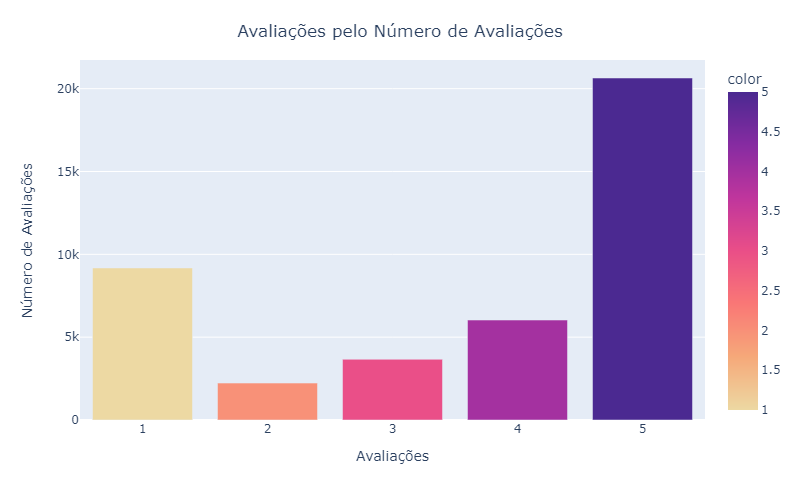
\includegraphics[trim={0cm 2cm 3cm 2cm},clip,scale=0.65]{./figs/eval.png}
    \caption{Distribuição das avaliações}
    \label{fig:evalDistribution}
\end{figure}

À primeira vista com o quantitativo de notas, é possível perceber que essa  distribuição é dada em forma de ``J" e é bastante típica em E-commerces. Grande  quantidade de avaliações 5, 4 e 1, pequena quantidade de 2 e 3.

Este tipo de distribuição pode ocorrer por várias razões. Uma possível explicação é que os clientes que estão extremamente satisfeitos ou insatisfeitos com um produto são mais propensos a deixar uma avaliação do que aqueles que têm uma experiência neutra. Isso pode resultar em uma concentração maior de avaliações com classificações muito altas ou muito baixas.

Outra possível explicação é que os clientes que têm uma experiência neutra com um produto podem não se sentir motivados a deixar uma avaliação. Eles podem sentir que o produto foi bom, mas não excepcional, e, portanto, não vale a pena dedicar tempo para escrever uma avaliação. Isso pode levar a um menor número de avaliações com classificações médias.

A distribuição em forma de ``J" das avaliações pode ser importante para as empresas entenderem, pois pode fornecer informações sobre a satisfação do cliente e a qualidade do produto. Se um produto tiver uma alta concentração de avaliações muito positivas, pode ser um indicador de forte satisfação do cliente e um produto de alta qualidade. No entanto, também é importante considerar o número de avaliações e a média geral das classificações, já que um pequeno número de avaliações pode distorcer a distribuição.

Seguidamente, plotou-se a distribuição binária das avaliações conforme foi seccionado na etapa de tratamento dos dados. De forma coerente com a \autoref{fig:evalDistribution} e com a divisão adotada, a maior parte das avaliações são positivas.

\begin{figure}[H]
    \centering
    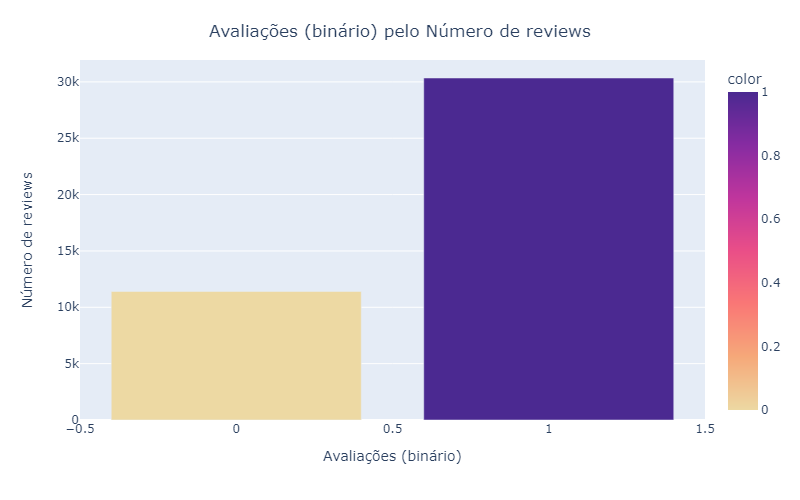
\includegraphics[trim={0cm 2cm 3cm 2cm},clip,scale=0.6]{./figs/bin_eval.png}
    \caption{Distribuição das avaliações binárias}
    \label{fig:binEvalDistribution}
\end{figure}

Uma nuvem de palavras então é gerada a partir de um conjunto de dados de texto referente aos comentários avaliativos dos clientes. As palavras são extraídas do texto e organizadas em uma nuvem, em que as palavras mais frequentes são maiores e as menos frequentes são menores. A nuvem de palavras pode ser usada para ajudar a identificar tópicos e padrões importantes em um conjunto de dados de texto e para comunicar visualmente essas informações.

\begin{figure}[H]
    \centering
    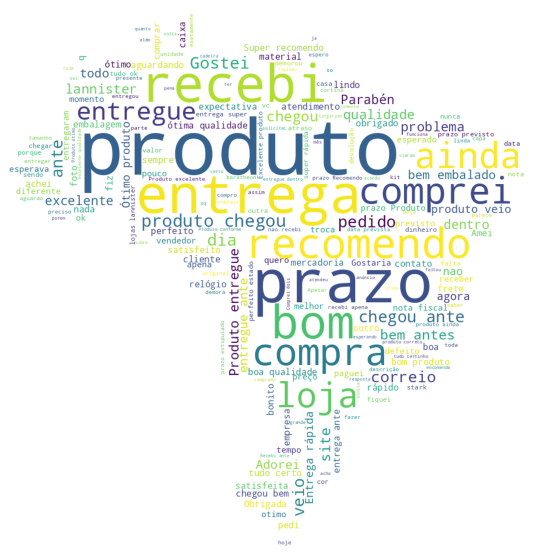
\includegraphics[scale=0.8]{./figs/word_cloud.png}
    \caption{Nuvem de palavras destacando os principais termos utilizados}
    \label{fig:wordCloud}
\end{figure}

Essa técnica visual pode ser usada em vários campos, incluindo análise de sentimentos, mineração de opiniões, análise de redes sociais, pesquisa de mercado e análise de feedback de clientes como o caso em específico. Além disso, por ser uma forma visualmente atraente de resumir informações e destacar pontos importantes, é bastante útil para relatórios e análises.

Tendo feito a tokenização das palavras, transformando-as em listas de numeros, filtrado pelas \textit{stopwords} e feito um processo de padronização textual, separou-se o dataset entre treino e teste e prosseguiu para as demais análises com os algorítmos de aprendizado de máquina e redes neurais.

Dentre os algoritmos de machine learning, encontrou-se as seguintes acurácias:

\begin{table}[H]
    \centering
    \begin{tabular}{l|ccccc}
        \hline
        { modelo}      & { Reg. Logística} & { F. Aleatórias} & { XGBoost} & { Naive Bayes} & lightGBM \\ \hline\hline
        { treino (\%)} & { 73.9}           & { 99.6}          & { 93.5}    & { 74.0}        & 86.7     \\\hline
        { teste (\%)}  & { 73.3}           & { 78.2}          & { 82.1}    & { 74.0}        & 81.3
    \end{tabular}
\end{table}

Observa-se que nos modelos XGBoost e lightGBM os valores foram muito próximos e apresentaram os melhores resultados em teste. Além disso, com as Florestas Aleatórias e XGBoost houve discrepâncias significativas entre as suas respectivas acurácias de treino e de teste. Essa diferença entre a acurácia (ou outra métrica de desempenho) é conhecida como a discrepância de generalização. Isso pode ter acontecido por diferentes motivos:

\begin{itemize}
    \item Overfitting: O modelo pode memorizar o conjunto de treinamento em vez de aprender os padrões subjacentes dos dados. Isso pode resultar em uma acurácia alta no conjunto de treinamento, mas uma acurácia baixa no conjunto de teste. Para evitar o overfitting, é importante usar técnicas como a regularização, a seleção de características e o aumento de dados.
    \item Diferenças entre os dados de treinamento e teste: Os dados de treinamento podem ser diferentes dos dados de teste, o que pode levar a discrepâncias na acurácia. Por exemplo, os dados de treinamento podem ter menos variabilidade do que os dados de teste, ou podem conter exemplos raros que não estão presentes no conjunto de teste.
    \item Tamanho do conjunto de dados: Quando o conjunto de dados é pequeno, é possível que a variação estatística nos resultados seja grande, levando a diferenças na acurácia entre o treinamento e teste.
\end{itemize}

É importante entender que uma discrepância de generalização não é necessariamente ruim, pois é possível que o modelo esteja apenas se adaptando aos dados de treinamento de forma mais eficaz. No entanto, se a discrepância for muito grande, pode ser um sinal de que o modelo precisa de ajustes. O objetivo é ter um modelo que generalize bem para novos dados e não apenas memorize os dados de treinamento.

Para a rede neural, plotou-se o gráfico da relação das \textit{epochs} pela acuracia do dataset de teste e de treino.
\begin{figure}[H]
    \centering
    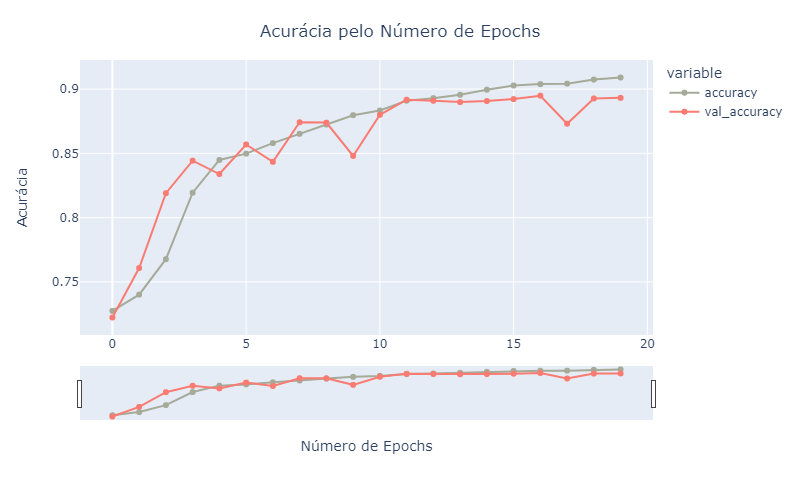
\includegraphics[scale=0.55]{./figs/lstm_acuracy.png}
    \caption{Relação acurácia por \textit{epochs}}
    \label{fig:lstmacuracy}
\end{figure}

Em redes neurais, uma \textit{epoch} refere-se a um ciclo completo de treinamento de todos os dados de treinamento disponíveis na rede. Durante cada um desses ciclos, os dados são passados pela rede em lotes (ou \textit{batch}), a rede faz previsões para cada lote, compara as previsões com as respostas corretas e atualiza os pesos e bias da rede para minimizar o erro (ou função de custo) entre as previsões e as respostas corretas.

Após uma \textit{epoch} completa, a rede é capaz de fazer previsões melhores do que antes do treinamento começar. À medida que o treinamento continua avançando, as previsões melhoram gradualmente até que a rede esteja suficientemente treinada para fazer previsões precisas sobre novos dados.

O número de \textit{epochs} que uma rede neural precisa para ser treinada depende do problema e da complexidade da rede. Um número muito baixo de \textit{epochs} pode resultar em previsões imprecisas, enquanto um número muito alto pode levar a um excesso de ajuste (overfitting) dos dados de treinamento.

Por fim, faz-se um comparativo entre a acurácia de todos os modelos para o dataset de treino e tem-se a \autoref{tab:time} com o tempo de execução para cada um dos modelos.

\begin{figure}[H]
    \centering
    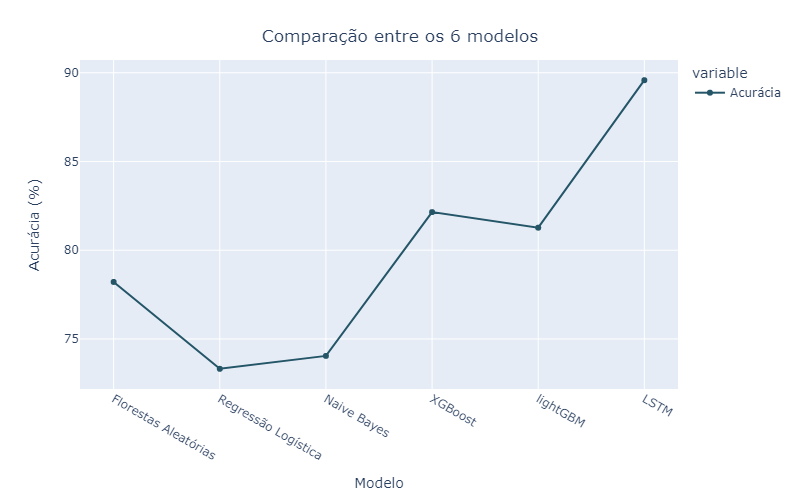
\includegraphics[scale=0.55]{./figs/comparative.png}
    \caption{Comparação de acurácia entre modelos}
    \label{fig:comparative}
\end{figure}

\begin{table}[H]
    \centering
    \small
    \begin{tabular}{c|cccccc}
        \hline
        { modelo}        & { Reg. Logística} & { F. Aleatórias} & { XGBoost} & { Naive Bayes} & lightGBM & LSTM \\ \hline \hline
        { Tempo (s)}     & { 21.5}           & { 1.5}           & { 3.0}     & { 0.1}         & {1.8}    & 1500 \\ \hline
        { Acurácia (\%)} & { 73.3}           & { 78.2}          & { 82.1}    & { 74.0}        & 81.3     & 90.0 \\
    \end{tabular}
    \caption{Tempo de execução/Acurácia dos modelos avaliados em teste}
    \label{tab:time}
\end{table}

Embora a acurácia seja uma métrica importante, ela pode não ser suficiente para avaliar completamente o desempenho de um modelo em alguns casos. Por exemplo, em problemas de classificação desbalanceados, onde uma classe é muito mais comum do que a outra, a acurácia pode ser enganosa. Nesses casos, outras métricas, como a precisão, a recall e a F1-score podem ser mais úteis.

Além disso, a acurácia não leva em consideração a gravidade dos erros de classificação. Por exemplo, em um problema de diagnóstico médico, um falso negativo pode ter consequências mais graves do que um falso positivo. Portanto, é importante avaliar o desempenho do modelo em relação a métricas que levam em consideração a gravidade dos erros de classificação, como a matriz de confusão.

Isso posto, avaliou-se os modelos também pela matriz de confusão e curva ROC.


\begin{figure}[H]
    \centering
    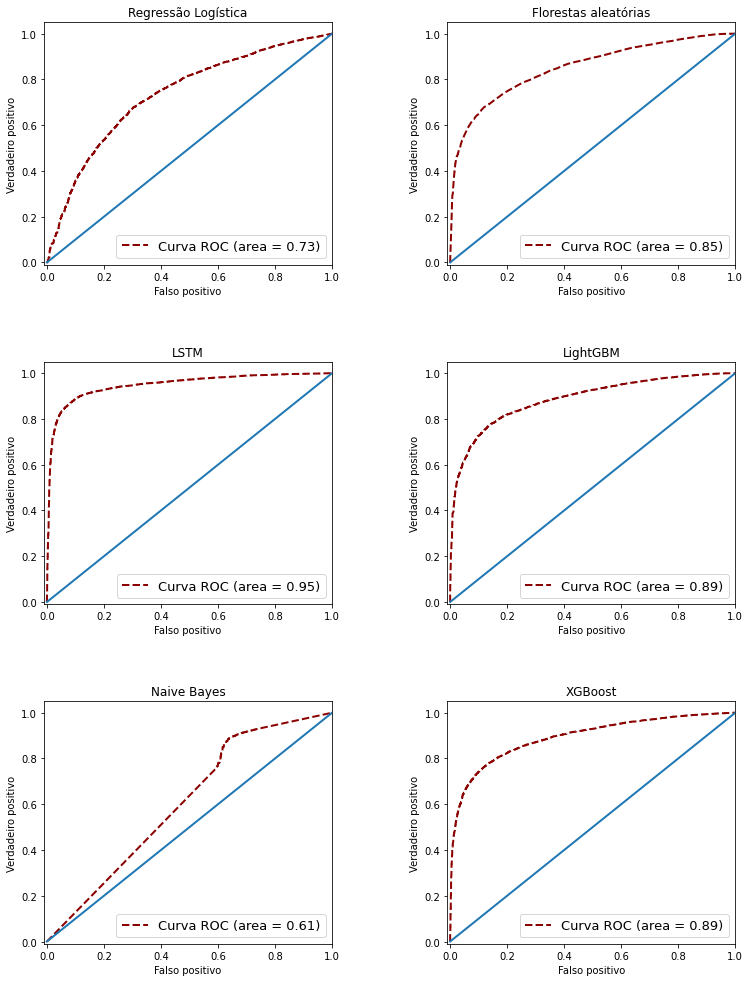
\includegraphics[scale=0.6]{./figs/roc_v.png}
    \caption{Curvas ROC dos modelos utilizados}
    \label{fig:roccurve}
\end{figure}

\begin{figure}[H]
    \centering
    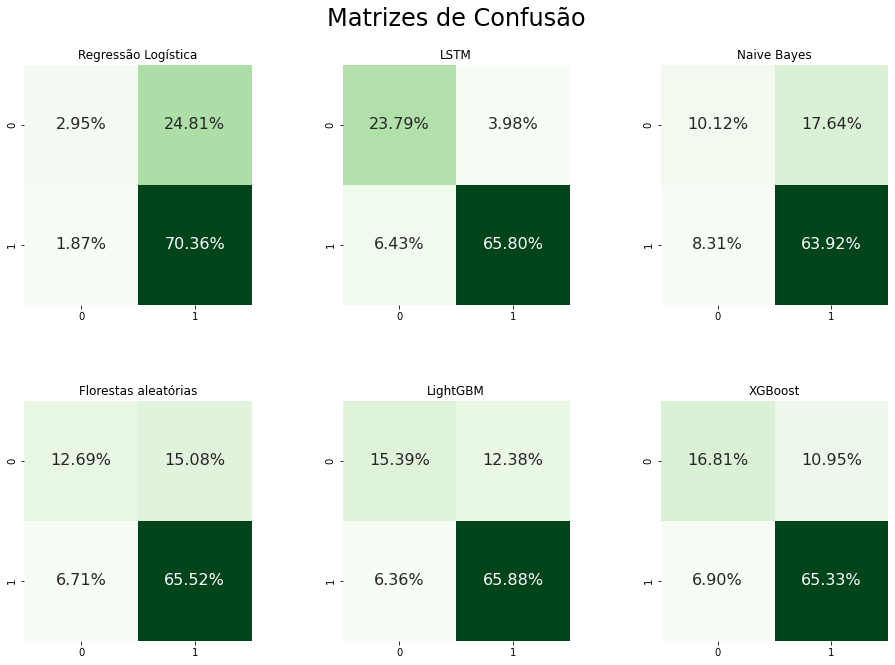
\includegraphics[scale=0.5]{./figs/confusion.png}
    \caption{Matrizes de confusão dos modelos utilizados}
    \label{fig:mconfusion}
\end{figure}

A matriz de confusão é uma tabela que mostra o número de exemplos que foram classificados corretamente e incorretamente pelo modelo, divididos em quatro categorias: verdadeiro positivo (TP-00), verdadeiro negativo (TN-11), falso positivo (FP-10) e falso negativo (FN-01). A partir dessa matriz, várias métricas de desempenho podem ser calculadas, incluindo a acurácia, precisão e recall. A matriz de confusão pode ajudar a identificar padrões de erros comuns que o modelo está cometendo.

Já a curva ROC (Receiver Operating Characteristic) é uma curva que mostra a relação entre a taxa de verdadeiros positivos (TPR) e a taxa de falsos positivos (FPR) para diferentes valores de limiar de classificação. Em outras palavras, a curva ROC mostra como o modelo se comporta em termos de sensibilidade e especificidade para diferentes pontos de corte de probabilidade de classificação. Quanto mais próxima a curva ROC estiver do canto superior esquerdo, melhor será o desempenho do modelo. A área sob a curva ROC (AUC-ROC) é uma medida resumida da performance do modelo, sendo que o valor máximo é 1,0, o que indica uma performance perfeita.

A escolha entre usar a matriz de confusão e/ou a curva ROC depende do objetivo do problema e da preferência do usuário. Enquanto a matriz de confusão oferece informações detalhadas sobre o desempenho do modelo em cada classe, a curva ROC pode ser mais útil para escolher o melhor modelo entre vários modelos ou ajustar o ponto de corte de classificação para atingir um determinado objetivo, como minimizar a taxa de falsos positivos ou maximizar a taxa de verdadeiros positivos.

